% Appendix B

\chapter{系统构建} % Main appendix title
\label{AppendixB} % For referencing this appendix elsewhere, use \ref{AppendixA}
\section{模型功能和系统实现}

本项目所有代码和文档开源于 Project-Unicom \quad \url{https://github.com/BigDataSystemTHU2018/Project-Unicom}

\subsection{系统架构}
如图(\ref{fig:pattern})所示,整体模型架构分为数据预处理和预分析,模型构建,结果可视化和后分析三个层次。
\begin{figure}[ht]
\centering
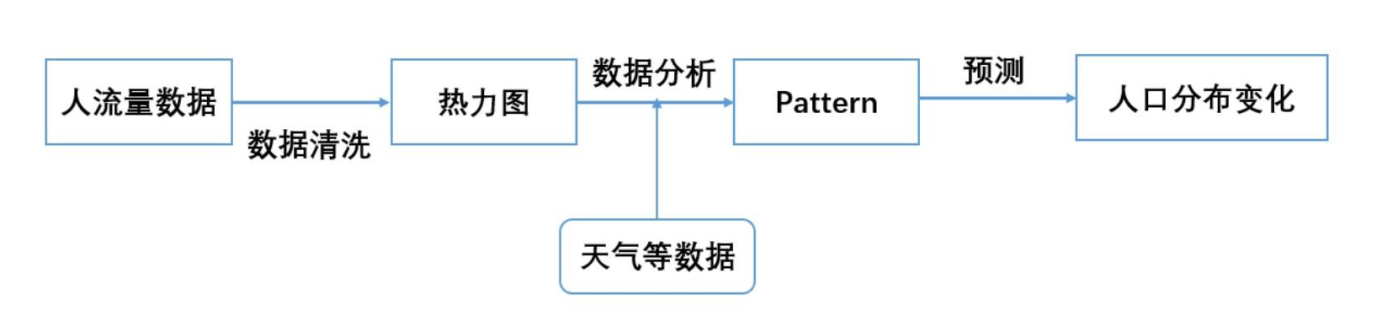
\includegraphics[width=0.8\textwidth]{pattern.png}
\caption{项目分析思路}
\label{fig:pattern}
\end{figure}
